\documentclass[a4paper,12 pt]{report}
\usepackage{latexsym}
\usepackage[utf8]{inputenc}



%\usepackage[english]{babel}
\usepackage[italian]{babel}

\usepackage[protrusion=true,expansion=true]{microtype}	
\usepackage{amsmath,amsfonts,amsthm} % Math packages
\usepackage[pdftex]{graphicx}	
\usepackage{mathtools}

\usepackage{hyperref}
\usepackage[table,xcdraw]{xcolor}
\usepackage{setspace}
\usepackage{amssymb}
\usepackage{listings}
\usepackage{url}

\usepackage{xcolor}
\usepackage[T1]{fontenc}
\newcommand\myworries[1]{\textcolor{red}{#1}}

\usepackage{enumitem}
\usepackage{float}
\usepackage{hyperref}
\usepackage{tikz}
\usepackage{multirow}
\usepackage{todonotes}
\usepackage{placeins}

\usepackage{graphicx}  
\usepackage{array}
\usepackage{booktabs} 
\usepackage{pifont}
\newcommand{\xmark}{\ding{55}}
\newcommand{\cmark}{\ding{51}} 

\usepackage[square,numbers]{natbib}

%per pseudocodice
\usepackage{algorithm} 
\usepackage{algorithmic}
\floatname{algorithm}{Algoritmo}
\renewcommand{\thealgorithm}{\unskip}
\newlength\myindent
\setlength\myindent{2em}
\newcommand\bindent{%
	\begingroup
	\setlength{\itemindent}{\myindent}
	\addtolength{\algorithmicindent}{\myindent}
}
\newcommand\eindent{\endgroup}
\usepackage{listings}
% package italiano
%
% Opzionale
%
%\renewcommand{\contentsname}{Sommario}
%\renewcommand{\listfigurename}{List of Figures}
%\renewcommand{\listtablename}{List of Tables}
%\renewcommand{\bibname}{Bibliografia}
%\renewcommand{\indexname}{Indice}
%\renewcommand{\figurename}{Figura}
%\renewcommand{\tablename}{Tavola}
%\renewcommand{\partname}{Parte}
%\renewcommand{\chaptername}{Capitolo}
%\renewcommand{\appendixname}{Appendice}
%\renewcommand{\abstractname}{Abstract}
%\renewcommand{\footnotesize}{\scriptsize}
%\renewcommand{\today}{\ifcase\month\or
%  Gennaio\or Febbraio\or Marzo\or Aprile\or Maggio\or Giugno\or
%  Luglio\or Agosto\or Settembre\or Ottobre\or Novembre\or Dicembre\fi
%  \space\number\day, \number\year}

% package formato
\pagestyle{plain}
\setlength{\topmargin}{0.0in}
\setlength{\headheight}{0.1in}
\setlength{\headsep}{0.0in}
\setlength{\footskip}{0.8in}
\setlength{\textheight}{9.0in}
\setlength{\textwidth}{6.0in}
\setlength{\oddsidemargin}{0.2in}
\setlength{\evensidemargin}{0.2in}
\setlength{\parindent}{0.4 in}
\onehalfspacing


\def\cent{\centerline}
\def\vs{\vskip 10 pt plus 1 pt}
\def\bs{\bf}
\def\grad{\vec{\nabla}}
\def\gradx{\vec{\nabla}_x}
\def\epsilon{\varepsilon}



\newcommand{\cvd}{\begin{flushright}$\Box$\end{flushright}}
\newcommand{\tr}{{\rm Tr}\;}
\newcommand{\eq}{\begin{equation}}
\newcommand{\feq}{\end{equation}}
\theoremstyle{definition}
\newtheorem{definition}{Definition}[section]
 
\theoremstyle{remark}
\newtheorem*{remark}{Remark}

\definecolor{blu_dmi}{HTML}{002e62}


%%%%%%%%%%%%%%%%%%%%%%%%%%%%%%%%%
%%%%%%%%%%%%%%%%%%%%%%%%%%%%%%%%%
%%%%%%%%%%%%%%%%%%%%%%%%%%%%%%%%%
%%%%%%%%%%%%%%%%%%%%%%%%%%%%%%%%%



\begin{document}
    % Thesis frontmatter --------------------------------------------

\thispagestyle{empty} %suppress page number

	\noindent % just to prevent indentation narrowing the line width for this line
	
\includegraphics[width=0.15\textwidth]{img/logoUniPg}
	\begin{minipage}[b]{0.7\textwidth}
		\centering
		{\Large{\textsc{Universit{\`a} di Perugia}}}\\
		\vspace{0.4 em}
		{\large {Dipartimento di Matematica e Informatica}}
		\vspace{0.6 em}
	\end{minipage}%
	
\includegraphics[width=0.15\textwidth]{img/logoDMI}
	
	\vspace{8 em}

	\begin{center}
		

	
		{\Huge{Appunti Knowledge Representation and Automated Reasoning }}\\
		\vspace{2 em}
		{\large { Autore: Chiara Luchini}}\\
		\vspace{5 em}
		{\large {Basati su:}}\\
		{\large {- Slides del Prof. Stefano Bistarelli}}\\
		{\large {- Lezioni del Prof. Stefano Bistarelli}}\\
		%{\large \textcolor{blu_dmi}{- Appunti lezioni online Prof. Alfredo Navarra}}\\
		
	
	

%		\makebox[380pt][c]{\textcolor{blu_dmi}{\textit{Advisor} \hfill \textit{}}}
%		\makebox[380pt][c]{\textcolor{blu_dmi}{\textbf{Dott. Francesco Santini \hfill}}}
		
		\vspace{6 em}
		\vfill
		
	{\rule{380pt}{.4pt}}\\
		\vspace{1.2 em}
		\large{{Anno Accademico 2021/2022}}
		
		
		
		
	\end{center}

% ------------------------------------------------------------------
    \newpage
  	\tableofcontents
    \newpage
    %\lstlistoflistings
	\newpage
	\listoffigures
    \newpage
    \chapter{Reati informatici}
Il rapporto tra informatica e diritto è iniziato in Italia, salvo sporadici ed occasionali interventi, nel lontano 1993 quando, grazie alla legge 547 del 1993 il codice penale ed
il codice di procedura fecero la conoscenza di termini come “sistema informatico”, “programmi per elaboratori”, "elaboratori”,“parole chiave” i reati informatici entravano a far parte del nostro ordinamento. 
La definizione più precisa di reato informatico è quella secondo cui 
\begin{center}
 \textbf{il crimine informatico rappresenta qualsiasi atto o fatto contrario alle norme penali, nel quale il computer è stato coinvolto come oggetto o strumento}   
\end{center}
Perché si possa parlare di "reato informatico" la presenza di un computer è un elemento essenziale ma non sufficiente, non basta che il computer sia presente, \textbf{ma questo deve anche svolgere un ruolo rilevante  nel crimine.} \\
Innanzitutto dobbiamo distinguere tra \textbf{reati informatici proprio ed impropri} a seconda che il computer rappresenti un elemento essenziale del reato, ovvero soltanto un semplice strumento:
\begin{itemize}
    \item \textbf{reati informatici propri}: reati concepibili solo ai danni di un computer o di una rete telematica;
    \item \textbf{reati informatici impropri}: reati elaborati per il mondo reale ma realizzabili anche attraverso internet.
\end{itemize}

\chapter{Acquisizione e sequestro della prova informatica}
\section{Fasi dell'acquisizione di prove }
Parlando di “evidenze digitali” dobbiamo distinguere tra la fase di acquisizione, di conservazione, di trattamento, di analisi, di esposizione e di relazione delle stesse. Per semplice comodità e ben consapevoli che si tratta di una distinzione fittizia, ora distingueremo le varie fasi. 

\subsection{Raccolta delle prove}
Spesso alcune prove vengono raccolte prima di entrare in contatto con la persona sottoposta ad indagine quali prove dipende in massima parte dal tipo di indagine dal tipo di crimine e dagli strumenti forniti all’uopo dal legislatore. Un'ulteriore distinzione deve essere fatta tra\textbf{ reati permanenti} (i.e. realizzazione di un sito web) e \textbf{reati istantanei} (i.e. ingiurie effettuate in chat, condivisione di materiale pedo) in quanto differenti sono le tracce lasciate dagli autori. Tuttavia ci sono delle caratteristiche comuni:
\begin{itemize}
    \item  particolare esigenza di \textbf{celerità} nell'acquisizione di prove, basta poco per alterarle volontariamente o involontariamente;
    \item l'investigatore deve conoscere bene le modalità con cui è stato commesso il reato, in quanto vi può essere una notevole differenza nel valore degli elementi di prova raccolti a seconda delle azioni del criminale.
\end{itemize}
Allo stesso modo, quando si procede all'acquisizione di dati specifici i dati acquisiti dovranno essere conservati in un supporto non modificabile, per esempio CD ROM o DVD ROM, e, possibilmente, firmati con firma digitale o, in alternativa, una volta “ il supporto ne dovrà essere acquisito l' hash. L'Hash dovrà essere riportato nel verbale.

\subsection{Perquisizione ed ispezione}
Di fronte ad un computer il codice ci consente di scegliere due differenti strade l'ispezione o il sequestro, ma è comunque necessario procedere all'analisi dello stesso.
\subsubsection{Casi e forme delle ispezioni}
L'ispezione delle persone, dei luoghi e delle cose è disposta con decreto motivato quando occorre accertare le tracce e gli altri effetti materiali del reato. Se il reato non ha lasciato tracce o effetti materiali, o se questi sono scomparsi o sono stati cancellati o dispersi, alterati o rimossi, l'autorità giudiziaria descrive lo stato attuale e, in quanto possibile, verifica quello preesistente, curando anche di individuare modo, tempo e cause delle eventuali modificazioni. L'autorità giudiziaria può disporre rilievi segnaletici, descrittivi e fotografici e ogni altra operazione tecnica anche in relazione a sistemi informatici o telematici, adottando misure tecniche dirette ad assicurare la conservazione dei dati originali e ad impedirne l'alterazione.
\subsubsection{Casi e forme delle perquisizioni}
Quando vi è fondato motivo di ritenere che taluno occulti sulla persona il corpo del reato o cose pertinenti al reato  è disposta \textbf{perquisizione personale}. Quando vi è fondato motivo di ritenere che tali cose si trovino in un determinato luogo  ovvero che in esso possa eseguirsi l'arresto dell'imputato o dell'evaso, è disposta \textbf{perquisizione locale }. Quando vi è fondato motivo di ritenere che dati, informazioni, programmi
informatici o tracce comunque pertinenti al reato si trovino in un sistema informatico o telematico, ancorché protetto da misure di sicurezza, ne è disposta la perquisizione, adottando misure tecniche dirette ad assicurare la conservazione dei dati originali e ad impedirne l'alterazione.
\\
La perquisizione rappresenta un momento fondamentale dell'indagine, soprattutto per la labilità e la deperibilità delle prove informatiche eventuali reperti non individuati in prima battuta sono, probabilmente, destinati a sparire in maniera definitiva. Proprio per tale ragione, nel corso della perquisizione non ci si dovrebbe mai accontentare dei risultati trovati facilmente o consegnati spontaneamente, ma è necessario operare per verificare se vi sono componenti hardware nascosti. Occorre poi verificare l'eventuale presenza di un server di raccolta dati eventualmente accessibile tramite Wi Fi. 
\paragraph{Rilevare un NAS.}  Grazie alle capacità wireless i dischi operano sia come punto d'accesso Wi Fi sia come un nodo Wi Fi e, potendo essere visti ed utilizzati in rete, possono essere usati per conservare file di vario genere. In alternativa è anche possibile utilizzare un portatile dotato di connessione wi fi ed amministrato da remoto per svolgere tutta l'attività “. L'unico modo per individuare simili dispositivi è quello di disporre, in sede di perquisizione, di un sistema in grado di effettuare un'analisi della rete alla ricerca di
altri dispositivi collegati. Una volta individuati eventuali " sospetti è necessario annotare il MACADDRESS ed andarli a cercare uno per uno per verificare se si tratta di un server NAS, di un computer remoto o di un semplice access point.
\\
Tutte le operazioni devono essere condotte in modo da \textbf{“cristallizzare"} le prove evitando ogni possibile contaminazione degli elementi probatori per esempio MAI accendere i computer individuati ed annotare con cura, anche scattando fotografie, la disposizione degli apparati all'interno dell'ufficio o dell'abitazione. Prescindendo dagli aspetti pratici della perquisizione, soffermiamoci sull'esigenza di acquisire i supporti informatici senza correre il rischio di alterarne in alcun modo il contenuto.  In caso di \textbf{computer spento}, nulla quaestio l\textbf{o si imballa}, apponendo i sigilli alla scatola, e lo si porta via, ma l'esperienza insegna che, sempre più spesso, i PC rimango costantemente accesi. In caso di \textbf{computer acceso} la soluzione ottimale sarebbe poter disporre, direttamente in sede di perquisizione, di un \textbf{soggetto con adeguata competenza} che possa procedere ad una \textbf{sommaria analisi} della macchina (annotando tutte le operazioni eseguite) per poi spegnerla in maniera sicura ma nel caso in cui ciò non fosse possibile, la dottrina più autorevole sostiene che, p\textbf{resa nota delle informazioni visualizzate} sul monitor e scattate fotografie dello stesso si deve \textbf{staccare direttamente la spina} dal computer procedendo anche alla rimozione delle batterie in caso di computer portatile. In questo modo si perde la possibilità di acquisire i dati presenti in RAM, ma allo stato delle cose si tratta della procedura più sicura per personale non qualificato.


\subsection{Catena di custodia}
Una volta acquisiti gli elementi presenti deve essere compilato un modulo noto come “catena di custodia” in cui vengono indicati espressamente tutti i soggetti entrati in contatto con le prove e tutte le operazioni compiute sulle stesse. 

\subsection{Perquisizione e sequestro}
Il nodo centrale della questione è “in caso di indagini per reati informatici, è necessario sequestrare tutto il materiale trovato, tutto il computer, solo l'hard disk oppure è sufficiente acquisire una copia dei dati?”. Dobbiamo osservare che non può esserci una risposta precisa a questa domanda in quanto a reati differenti devono corrispondere differenti tipologie di indagine che richiedono approcci molto diversi. In ogni caso dovrà essere preferita una modalità di acquisizione meno invasiva e che comporta il minor danno per il soggetto che la subisce.
Il mancato sequestro di un componente secondario potrebbe pregiudicare la possibilità di svolgere ulteriori accertamenti.  Per esempio il mancato sequestro della tastiera, del mouse o dello stesso mouse pad potrebbe
rendere impossibile verificare eventuali tracce che, soprattutto in casi particolari, potrebbero servire per individuare in maniera precisa l'autore del reato arrivando magari anche a scagionare l'iniziale imputato. Inoltre l'acquisizione di copia dei dati immediatamente, direttamente in sede di perquisizione, presenta altri due grossi problemi:
\begin{enumerate}
    \item richiede, per essere eseguita, la presenza di personale particolarmente esperto in grado di operare, in maniera sicura, su supporti hardware e software sconosciuti e di individuare, in tempi rapidissimi tutti i file di interesse probatorio 
    \item L'operazione, anche se eseguita secondo le best practices della computer forensics , è, di fatto, irripetibile in quanto il materiale, rimasto nella disponibilità dell'imputato, deve considerarsi non più utile per finalità investigative.
\end{enumerate}
In breve l'utilizzo dello strumento dell'ispezione, con la conseguente acquisizione, mediante masterizzazione, dei soli file pertinenti al reato, andrebbe utilizzata soltanto laddove il computer assuma la veste di mero contenitore della prova del crimine e si ritenga opportuno non operare un sequestro, per esempio perché lo si ritiene sproporzionato al fatto contestato, oppure nel caso di attività presso terzi estranei di fatto alla vicenda. Una buon compromesso è rappresentato dal sequestro del solo hard disk (oppure dall'acquisizione, con strumenti idonei, di un'immagine dello stesso). Tale soluzione, applicabile alla maggior parte dei reati informatici, consente un pieno controllo del contenuto del supporto e la ripetibilità, in qualsiasi momento,
dell'analisi eseguita. Di contro richiede, direttamente in sede di perquisizione e l'hard disk senza danneggiarlo e, soprattutto, in grado di verificare la presenza di dispositivi in grado di impedire l'accesso ai dati in esso contenuti come, ad esempio, nel caso della tecnologia ABIT Secure IDE o similari. In tal caso è buona norma acquisire \textbf{l'hash} dell'hard disk prima e dopo la copia, stamparlo e farlo sottoscrivere alla controparte in questo modo sarà possibile dimostrare che la prova non è stata alterata in alcun modo.  In ogni caso una volta che il PC è stato spento non deve essere più riavviato, anzi sarebbe buona norma scollegare eventuali cavi di alimentazione e, nel caso dei portatili, rimuovere le batterie. Tutte le operazioni devono essere annotate e deve essere mantenuta una precisa catena di custodia in grado di dimostrare ogni passaggio delle evidenze informatiche. 
\subsubsection{L'hash}
L'hash, \cite{hash-informatica-forense}, è una funzione matematica univoca ed unidirezionale (cioè non può essere invertita), che trasforma un testo di qualunque lunghezza (input) in testo di lunghezza fissa (output) relativamente limitata. In pratica, applicando una funzione di hash a un file o ad un intero hard disk, si ottiene una sequenza alfanumerica ad es. di 32 caratteri, che rappresenta una sorta di "impronta digitale" dei dati, e viene detta valore di hash. Le funzioni di hash presentano principalmente due proprietà interessanti dal punto di vista forense: \begin{itemize}
    \item è praticamente impossibile che due testi diversi abbiano lo stesso valore di hash o che, dato un valore di hash ricavato da un certo testo, si possa creare un testo differente che generi lo stesso hash
    \item è praticamente impossibile ricostruire il testo originario disponendo solo del valore di hash
\end{itemize}
Quindi, se i dati sui quali è stato calcolato il valore di hash cambiano anche di una sola virgola, il nuovo valore di hash sarà completamente diverso.
Quando si dice “praticamente impossibile” ci si riferisce al fatto che la probabilità che casualmente due testi differenti generino lo stesso hash è talmente bassa (per l’algoritmo MD5 siamo nell’ordine di $2^{64}$ tentativi) da divenire trascurabile, così come per ottenere un testo che generi un predeterminato valore di hash vi sono $2^{128}$ tentativi possibili.
Per quanto di interesse dell’informatica forense, possiamo dire che l’hash di un documento informatico e quello della sua copia bitstream, calcolati in sede di intervento presso il detentore con garanzia di contraddittorio, costituiscono (se uguali) una certificazione inoppugnabile che il contenuto del supporto “originale” è esattamente uguale alla “copia” sulla quale verranno effettuati gli accertamenti tecnici del caso.

\subsection{L'acquisizione}
In commercio è facile reperire programmi che consentono di creare un'intera partizione fat 32 o ntfs criptata in alcuni casi, la partizione può comprendere l'intero sistema operativo ed i relativi file di boot di swap, i file temporanei, eccetera ed è altresì possibile che tale partizione si avvii solo utilizzando un apposito dischetto In
assenza del floppy la partizione appare come spazio non formattato. In fase di analisi è bene ricordare che tutti gli accertamenti effettuati devono essere ripetibili per nessuna ragione il computer del sospetto dovrebbe essere avviato e,per nessuna ragione, le analisi dovrebbero essere effettuate utilizzando il materiale
originale e questo per due ottime ragioni:
\begin{enumerate}
    \item si rischia di danneggiare il supporto;
    \item si rischia di alterare il materiale.
\end{enumerate}
Dunque, per garantire la ripetibilità dell'analisi (vero principio cardine della computer forensics) è necessario operare su di una copia del supporto sequestrato. In commercio esistono numerosi prodotti, hardware e software, in grado di clonare un hard disk garantendo la non alterazione dell'originale e l'esatta corrispondenza originale copia. \'E buona norma anche procedere all'acquisizione della "firma" dell'intero supporto acquisito, con un'operazione detta hashing. L'operazione viene compiuta utilizzando un algoritmo MD5 che, generando un'impronta della lunghezza
di 128 bit (16 byte), costituisce un riferimento certo alla traccia originale, pur non consentendone la ricostruzione. Se si rendesse necessario avviare il computer, ad esempio nel corso di un'ispezione o per effettuare un'analisi preliminare, è necessario proteggere l'hard disk con un dispositivo FISICO che inibisca la scrittura sullo stesso write block o, in alternativa, utilizzare un apparato hardware per effettuare una copia precisa dell'hard disk ed avviare la macchina utilizzando la copia.

\subsection{ L'analisi}
\'E,quindi, importante che tutte le operazioni compiute siano tracciabili e possano essere adeguatamente giustificate e motivate. In genere l'analisi di un'evidenza digitale si svolge in tre fasi:
\begin{enumerate}
    \item la sua individuazione;
    \item la sua valutazione tecnica;
    \item la sua "contestualizzazione".
\end{enumerate}
Sulla base di questi elementi è, quasi sempre, possibile stabilire quando, come e perché un determinato file è comparso nell'hard disk. Un altro aspetto particolarmente interessante della computer's forensic è rappresentato dalla necessità di dar voce anche ai silenzi della macchina. Non è difficile, infatti, disponendo degli strumenti adeguati occultare un'immagine o un'intera partizione in modo che sia praticamente impossibile individuarla (come PGP Disk, TrueCript).  Dalla crittografia, scrittura cifrata, si è, infatti, passati alla steganografia scrittura
nascosta, ed il buon “ PGP Disk viene rapidamente sostituito da TrueCrypt che, per espressa previsione dei
programmatori, si basa sul principio della negazione plausibile viene creato un disco crittografato al cui interno se ne trova un altro.
\subsection{La relazione}
In premessa devono essere indicate tutte le attività svolte dal ricevimento del pacco fino all'acquisizione dell'immagine dei supporti. \'E possibile, ma non necessario, documentare mediante una videocamera la fase dell'acquisizione. In questa fase si deve offrire un riassunto del sistema analizzato e tutti quegli elementi di natura tecnica che possono rivelarsi utili in sede di analisi. Occorre individuare ed indicare programmi, file, cartelle riportando data di creazione, data di modifica e data di ultimo accesso. \'E necessario evidenziare ogni anomalia che si riscontri, soprattutto eventuali accessi al disco o ai dati SUCCESSIVI alla data del sequestro. Infine la relazione andrebbe conclusa con un paragrafo riepilogativo in cui si riepiloga quanto individuato e si traggono delle conclusioni.

\section{Errori comuni}
\begin{itemize}
    \item Avviare il PC e o installare l'hard disk rendendo l'accertamento NON ripetibile: inutilizzabilità della prova raccolta ai sensi del 360 cpp.
    \item Utilizzare programmi in grado di alterare le proprietà di file e cartelle (i.e. Antivirus) rendendo impossibile una corretta ricostruzione del comportamento del soggetto.
    \item Sindrome del veggente: trarre conclusioni o, peggio, fare affermazioni che non poggino su solide base oggettive. Distinguere sempre tra:
    \begin{itemize}
        \item prove: sono fatti o atti;
        \item indizi: solo se gravi, precisi e concordanti possono costituire una prova;
        \item presunzioni: l'operazione logica per cui da un fatto noto si risale ad un fatto ignoto.
    \end{itemize}
    \item Dare per scontato il risultato desiderato (colpevolezza o innocenza) omettendo di verificare la stabilità della relazione.
    \item Non verificare possibili alternative valide, logiche e plausibili.
    \item Utilizzare software pirata.
    \item Acquisire prove o informazioni in maniera illegale.
\end{itemize}

\chapter{Incident Response}
Come in ogni settore lavorativo, quindi, la sola componente proattiva non è sufficiente; i security incident possono verificarsi anche nella più corazzata delle strutture e quindi avere una divisione adibita al comportamento “reattivo” è ugualmente importante.

\begin{figure}[H]
	\centering
    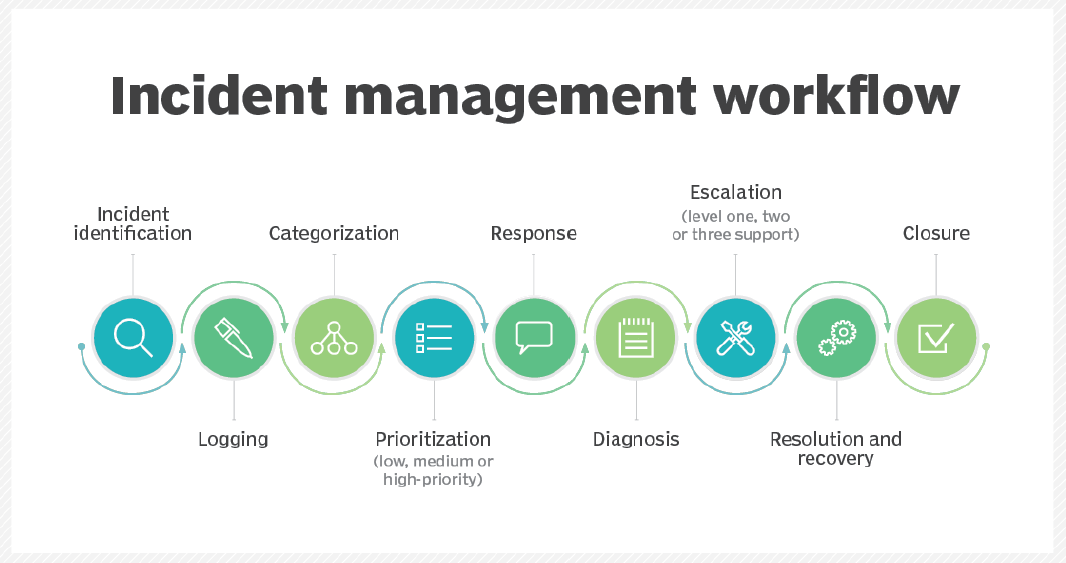
\includegraphics[width=15cm, keepaspectratio]{img/incident_response_fasi.png}
	\caption{Fasi Incident response, \cite{incident-response-immagine}.}\label{fig:incident_response}
\end{figure}

L’incident response \cite{incident-response}, cioè la risposta agli incidenti, è dunque un processo fondamentale all’interno di tale contesto e per tale motivo avere un team di persone adibite a questo scopo, opportunamente formate e dotate degli strumenti adeguati, è di vitale importanza per le aziende.
\section{Fasi dell'incident response}
\subsection{Identificazione dell'incidente}
\begin{itemize}
    \item Cosa sta succedendo?
    \item Abbiamo accesso a tutto il sistema informatico o dobbiamo interessare altri amministratori di rete o responsabili?
    \item Fermare l’attacco se è in corso
\end{itemize}

\subsection{Categorizzazione dell’incidente}
\begin{itemize}
    \item \'E un attacco mirato o casuale?
    \item Individuare tutti i dispositivi coinvolti
    \item Prima stima dei danni
\end{itemize}
\subsection{Risposta all’incidente}
\begin{itemize}
    \item Verifica della presenza di backup non compromessi
    \item Verifica degli accessi dai firewall per identificare un eventuale punto di ingresso
    \item Se viene individuato il punto di accesso, provvedere ad una copia fisica della memoria del dispositivo, compresa la RAM
\end{itemize}
\subsection{Soluzione dell'incidente}
\begin{itemize}
    \item Ripristino del sistema dai backup
\end{itemize}

\section{Problemi}
\begin{enumerate}
    \item Non sono stati fatti backup
    \item I backup sono compromessi
    \item I dati sono stati criptati
    \item Non si hanno privilegi di amministratore
    \item Non si hanno supporti dove memorizzare le copie fisiche degli HD
    \item I sistemi non prevedono desktop virtualizzati
    \item L’attaccante è ancora presente con sistemi di C\&C
    \item Il responder va in panico
    \item L’amministratore di rete non è raggiungibile
    \item Il sistema informatico non è ben strutturato
    \item Il sistema non riesce a tornare on line
    \item Sono stati compromessi dispositivi che si collegano a distanza
    \item I log dei firewall sono compromessi
    \item \'E stata usata come ingresso proprio la macchina dell’amministratore di rete
    \item \'E finito il caffè :)
\end{enumerate}

\section{Analisi dell'incidente}
\begin{itemize}
    \item Analisi dei file di log dei firewall
    \item Analisi dei dispositivi sicuramente compromessi
    \item Verifica dell’architettura della rete
    \item Verifica della tenuta dei backup
    \item Analisi di tutti i dispositivi in rete per verificare eventuali trojan
    \item Verifica dell’efficienza nella risposta all’incidente
\end{itemize}
 	\newpage
    % ...
    \bibliographystyle{plainnat}
    % Opzionale
    \newpage
    \bibliography{bibliografia}
	

    
\end{document}
